%\usepackage{appendix}
\chapter {Getting Started}
\thispagestyle{empty}
\label{chap4}

In this chapter we will get started with eSim. Referring to
this chapter will make one familiar with eSim and will help
plan the project before actually designing a circuit. 

\section{How to launch eSim?}
After the installation of eSim, a shortcut to eSim is created 
on the Desktop. To launch eSim double click on the shortcut.\\ 
Alternately, for Ubuntu Linux users, one can also launch eSim from the terminal.\\
1. Go to terminal.\\
2. Type \textbf{esim} and press {\tt Enter}.\\

The first window that appears is the workspace dialog as shown in 
\figref{workspace}. 
\begin{figure}[h]
\centering
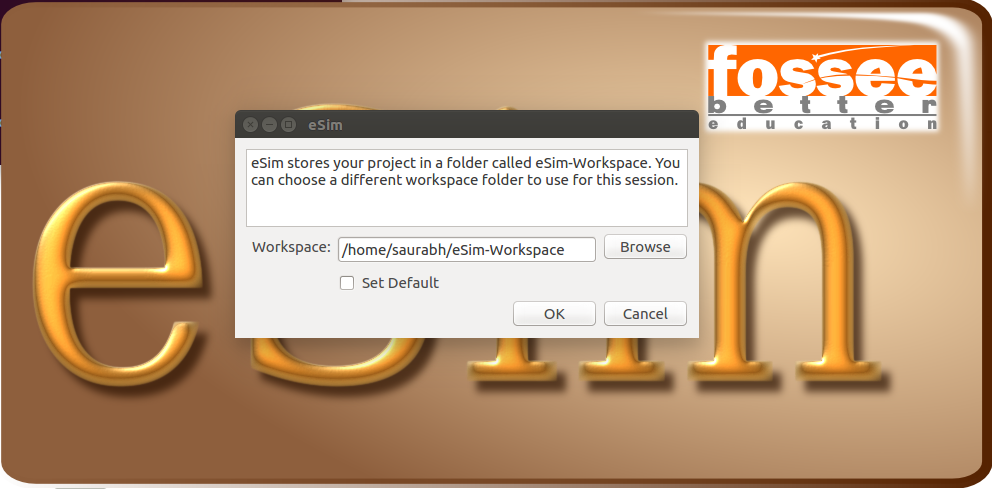
\includegraphics[width=\lgfig]{workspace.png} 
\caption{eSim-Workspace}
\label{workspace}
\end{figure}

\item 1.The default workspace is eSim-Workspace under home directory. 
To select a new workspace location, use the {\tt browse} option. Do not select a location which has a space character or special character(s). 
\item 2. If you select the \textbf{set default} click-box, then the chosen location will be set as default workspace and the dialog box won't appear next time you launch eSim.
\item 3. If you wish to change the default workspace location, then use the menu-bar from eSim's main Interface, which is explained in upcoming section.
\section{eSim User Interface}
The main graphic window of eSim is as shown in \figref{maingui}.
\begin{figure}[h]
\centering
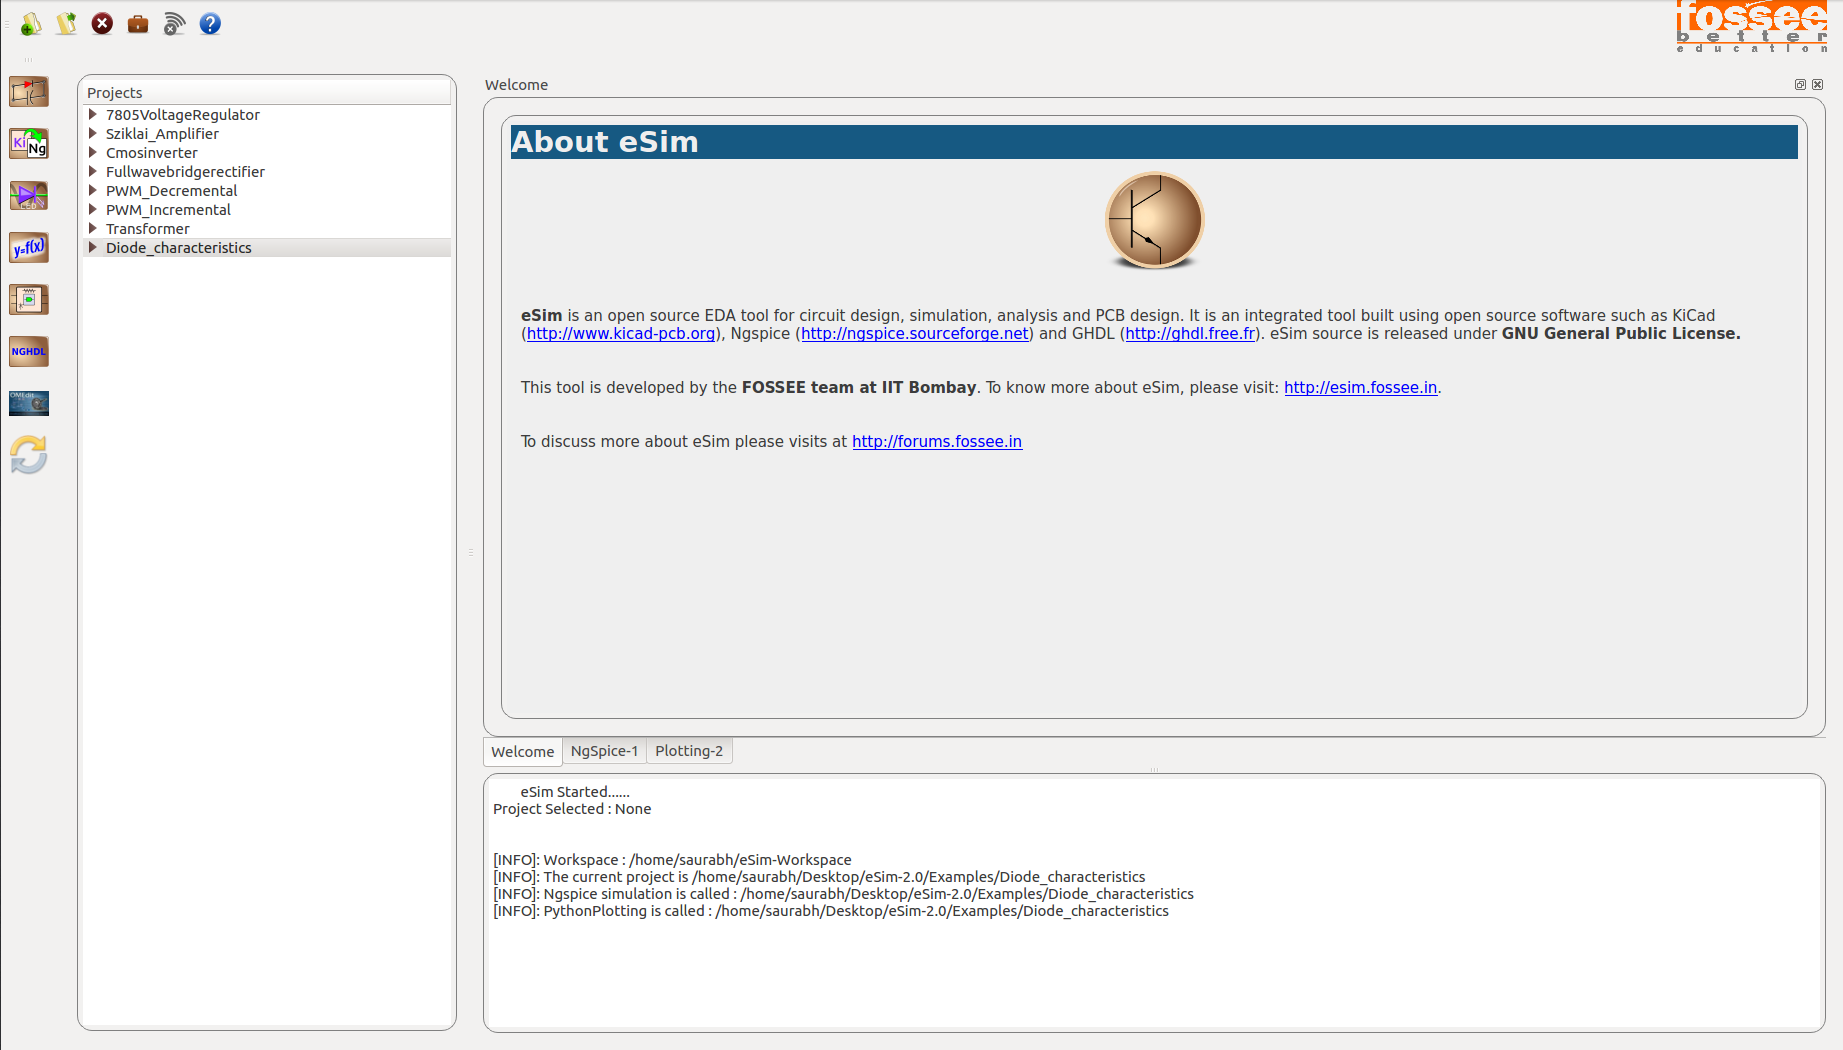
\includegraphics[width=\hgfig]{maingui.png}
\caption{eSim Main GUI}
\label{maingui}
\end{figure}
\\
The eSim window consists of the following sections.
\begin{enumerate}

\item Menubar
\item Toolbar
\item Project explorer
\item Dockarea
\item Console area
\end{enumerate}

\subsection{Menubar}
\begin{itemize}
\item \textbf{New Project}:
New projects are created in the eSim-Workspace. When this menu is selected, 
a new window opens up with {\tt Enter Project name} field. Type the name of 
the new project and click on {\tt OK}. A project directory will be created in 
eSim-Workspace. The name of this folder will be the same as that of the 
project created. \textit {Make sure that the project name does not have 
any spaces in between.} This project is also added to the project explorer.

\item \textbf{Open Project}:
This opens the file dialog of default eSim-Workspace where the projects are stored. 
Select the required project and click on {\tt Open}. The selected project is added 
to the project explorer.

\item \textbf{Close Project}:
This button closes the opened project.

\item \textbf{Change workspace} : Clicking on this will open the window shown in \figref{workspace}. If you have chosen a default workspace location but wish to change it later on, launch eSim, click on this icon and do the necessary changes. 

\item \textbf{Mode Switch} : Using this feature user can decide whether to fetch latest footprints(refer Section :PCB Designing) from the internet or use the locally available footprints. \\
Note : By switching to online mode, you will require a stable and high-speed internet connection, if it is not available to you then please always remain in the offline mode.

\item \textbf{Help} : Clicking on this icon will launch the eSim user manual for that particular version of eSim. 
\end{itemize}

\subsection{Toolbar}
The toolbar consists of the following buttons. See \figref{guitoolbar}.

\begin{figure}[h]
\centering
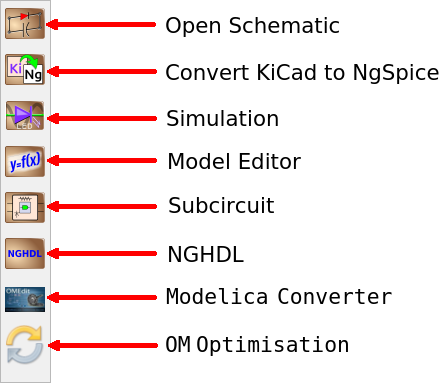
\includegraphics[width=\lgfig]{manual_images/guitoolbar.PNG}
\caption{Toolbar}
\label{guitoolbar}
\end{figure}

\subsubsection {Open Schematic}
The first button on the toolbar is the \texttt{Schematic
Editor}\index{Schematic!editor}. Clicking on this button 
will open the schematic editor. 
If  a new project  is  being  created, one will get a 
dialog box confirming the creation of a schematic. This 
is illustrated in See \figref{schematic-confirmation}. 
However, if an already existing project is opened, the 
schematic editor window is opened. To know how to use 
the schematic editor to create circuit schematics, refer 
to \chapref{chap5}. \\ \\
When one right clicks on a particular project : three options appear, their functions listed below: \\
\begin{enumerate}
    \item Rename Project : This will rename the project and the underlying files. Note that all project files must be closed from all running applications that access them before renaming a project.
    \item Remove Project : This will remove the project selected from the \texttt{Project Explorer} list.
    \item Refresh : At times, all the files under a project will not be displayed. In that case, selecting this option will update the latest files under a project. 
\end{enumerate}
\begin{figure}[h]
\centering
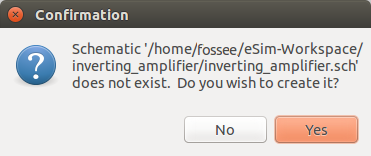
\includegraphics[width=\lgfig]{manual_images/schematic-confirmation.png}
\caption{Confirmation for schematic creation}
\label{schematic-confirmation}
\end{figure}

\subsubsection {Convert KiCad to Ngspice}
In the schematic editor window, after creating the schematic a netlist is to be  generated which contains information about the components present in the schematic created and their values specified . Although this netlist is present, it cannot be directly fed to the simulator. Here the KiCad-to-Ngspice converter comes into play.
This tool converts the netlist generated from the schematic into another netlist which is compatible with Ngspice, the simulator used in eSim.
The \textbf{Convert KiCad to Ngspice} window consists of five tabs namely \texttt{Analysis, Source Details, Ngspice Model, Device Modeling and Subcircuits}.
The details of these tabs are as follows.\\
\begin{itemize}
\item \texttt{Analysis:} This feature helps the user to enter the parameters for performing different types of analysis such as Operating point analysis, \index{Operating point analysis} DC analysis, \index{DC Analysis} AC analysis, \index{AC Small-signal Analysis} transient analysis, \index{Transient Analysis} DC Sweep Analysis. \index{DC Sweep Analysis}

It has the facility to select the
\begin{itemize}
    \item Type of analysis and
    \item The simulation parameter values for analysis
\end{itemize}

\item \texttt{Source Details:}eSim sources are added from {\tt eSim\_Sources} library in the \linebreak schematic. Sources such as \textit{SINE, AC, DC, PULSE, PWL} are in this library. The parameter values to all the sources added in the schematic can 
be given through 'Source Details' tab in the KiCad-To-Ngspice window.

\item \texttt{Ngspice Model:}Ngspice has in-built model such as \texttt{basic logic gates, \linebreak flip-flops, gain, summer, buffer, DAC and ADC block}etc. which can be utilised while building a circuit.
eSim allows to add and modify Ngspice model parameter through 
Ngspice Model tab.

\item \texttt{Device Modeling:}Devices like \texttt{Diode, JFET, MOSFET, IGBT, MOS} etc used in 
the circuit can be modeled using device model libraries. eSim also 
provides editing and adding new model libraries. While converting 
KiCad to Ngspice, these library files are added to the corresponding 
devices used in the circuit.

\item \texttt{Subcircuits:}eSim allows you to build subcircuits.  The subcircuits can again 
have components having subcircuits and so on. This enables users to 
build commonly used circuits as subcircuits and then use it across 
circuits. The subcircuits are added to the main circuits using this 
facility. We can also edit already existing subcircuits. 
\\
Once the values have been entered, press the {\tt Convert} button. This 
will generate the {\tt .cir.out} file in the same project directory.
Note that \textit{KiCad to Ngspice Converter} can only be used if 
the KiCad spice netlist {\tt .cir} file is already generated.
\\
\end{itemize}

\subsubsection {Simulation}
The netlist generated using the \texttt{KiCad to Ngspice} converter 
is simulated using \textit{Simulation} button on the eSim left toolbar. This
will run the Ngspice simulation for current project. eSim have two options 
to see the simulation output. The first one is the Python plotting window 
which opens up in the dock area, as shown in \figref{simulation-op}. 
The second is the Ngspice window with the simulation data. The user can 
type in Ngspice commands to view the plots. 

\textit {Note: If the user has used the plot components (available under eSim\_Plot library) at various nodes in the circuit schematic the Ngspice plots are displayed automatically.}

\begin{figure}[h]
\centering
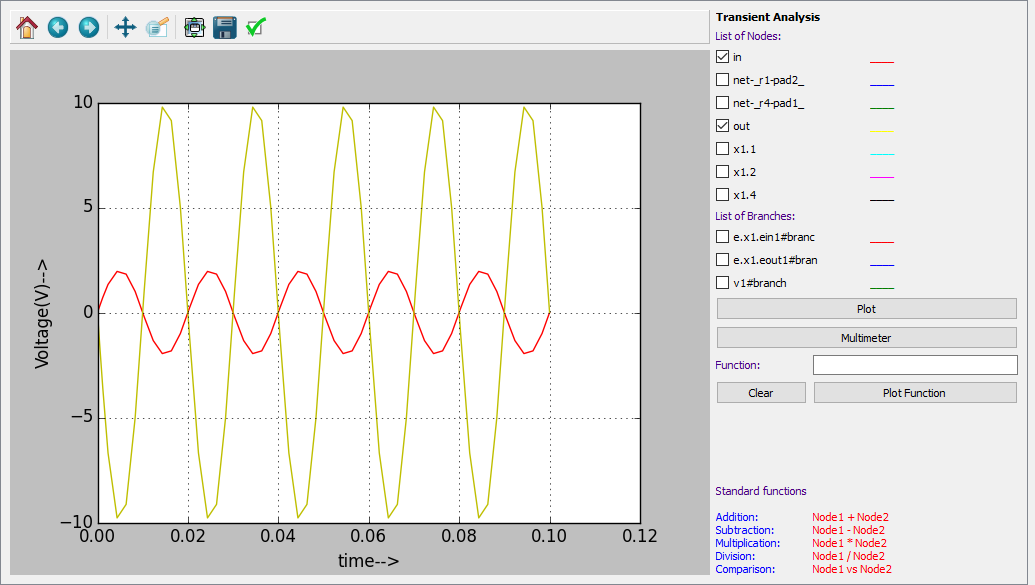
\includegraphics[width=\hgfig]{manual_images/simulation-op.png}
\caption{Simulation Output in Python Plotting Window}
\label{simulation-op}
\end{figure}

%\subsubsection {Foot Print Editor:}
%Clicking on the \textit{Footprint Editor} tool will open the {\tt CvPcb} 
%\index{CvPcb} window. This window will ideally open the .net file for the 
%current project. So, before using this tool, one should have the netlist 
%for PCB design (a .net file). %To know more about how to assign footprints 
%to components, see \chapref{chap7}.

%\subsubsection {PCB Layout:}
%Clicking on the \textit{Layout Editor} tool will open {\tt
%Pcbnew}\index{Pcbnew}, the layout editor used in eSim. In this
%window, one will create the PCB. It involves laying tracks and vias,
%performing optimum routing of tracks, creating one or more copper
%layers for PCB, etc. It will be saved as a {\tt .brd} file in the 
%current project directory. %\chapref{chap7} explains how to use the 
%\textit{Layout Editor} to design a PCB. 

\subsubsection {Model Editor}
eSim also gives an option to re-configure the model library of a
device. It facilitates the user to change model library of devices
such as diode, transistor, MOSFET, etc. It also facilitates the user to load the spice library externally and use it for the existing or newly added models.To know
more about Model Editor, refer to \chapref{chap7}.

\subsubsection {Subcircuit}
eSim also allows the user to build subcircuits. The subcircuits can
again have components having subcircuits and so on. This enables users
to build commonly used circuits as subcircuits and then use it across
circuits. For example, one can build an Op-Amp as a
subcircuit and then use it as just a single component across circuits
without having to recreate it. Clicking on \textit{Subcircuit
Builder} tool will allow one to edit or create a subcircuit. To know
how to make a subcircuit, refer to \chapref{chap8}.

\subsubsection {NGHDL}
NGHDL is an add on to eSim for mixed signal circuit simulation. By using the foreign language interface of GHDL, NGHDL communicates with Ngspice and accomplishes mixed signal simulation. Using NGHDL, user can create custom digital model using VHDL language. From simple multiplexers, counters to microcontrollers and ASICs, any custom component in the digital domain can be realized using the NGHDL tool. The created digital model can be used in either mixed signal circuit or a standalone circuit operating in digital domain. NGHDL gives user the liberty to edit existing models supplied with eSim per their needs, either for experimenting new ideas or to change the model per their specific requirement.

\subsubsection {Modelica Converter}
OpenModelica (OM) is an open source modeling and simulation tool based on
Modelica language. Modelica is an object oriented language. The Modelica Converter in eSim interface, converts the ngspice netlist to Modelica format. This facility will be only available if you have OpenModelica already installed in the system. More details on how to use this module is available in \chapref{chap10}.

\subsubsection {OM Optimisation}
OMOptimisation (OMOptim) is a powerful and interactive tool for performing design optimisation. It has a good library of electrical components called Modelica Standard Library (MSL). OMOptim is stable and robust. It is very easy to add objective functions to the OMOptim interface.

\subsection{Project Explorer}
Project explorer contains the list of all the projects previously added to it. 
Select a project and double click on it, this will display all the files under 
this project. Right click on any displayed file to open it. To remove or refresh 
any project file from the project explorer, right click on the main project file.


\subsection{Dockarea}
This area is used to open the following windows.
\begin{enumerate}
    \item KiCad to Ngspice converter
    \item Ngspice plotting
    \item Python plotting
    \item Model builder
    \item Subcircuit builder
\end{enumerate}
Modules/Windows will appear here as per your selection.

\subsection{Console Area}
Console area provides the log information about the activity done during the current session.


